\documentclass[a4paper]{jpconf}
\usepackage{graphicx}
\begin{document}
\title{The CMS Data Aggregation System}

\author{Valentin Kuznetsov}
\address{Cornell University, Ithaca, New York, USA}
\ead{vkuznet@gmail.com}

\author{Dave Evans}
\address{Fermilab, Batavia, Illinois, USA}
\ead{evansde@fnal.gov}

\author{Simon Metson}
\address{Bristol University, Bristol, UK}
\ead{s.metson@bristol.ac.uk}


%In a large modern enterprise, information is almost inevitably distributed among several database management systems. Despite considerable attention from the research community, relatively few commercial systems have attempted to address this issue. This article describes the technology that enables clients of IBM's federated database engine to access and integrate the data and specialized computational capabilities of a wide range of relational and non­relational data sources.

\begin{abstract}
%A meta-data plays significant role in a large modern enterprises, research experiments,
%digital libraries where it comes from different sources and distributed in a 
%variety of forms and digital formats. It is organized and managed by constantly
%evolving software using both relational and non-relational data sources. There is
%a big demand to enable information discovery from multiple sources.
%Here we discuss a new data aggregation system which consume and deliver information 
%from different relational and non-relational data sources on a concrete example 
%of large scale, distributed system of CMS physics experiment at LHC.

Meta-data plays significant role in a large modern enterprises, 
research experiments, digital libraries where it comes from different 
sources and distributed in a variety of forms and digital formats. 
It is organized and managed by constantly evolving software using 
both relational and non-relational data sources. There is a big 
demand to enable information discovery from multiple sources.

Here we discuss a new data aggregation system which consumes, 
indexes and delivers information from different relational and 
non-relational data sources to answer cross data source queries 
examining metadata associated to petabytes of 
experimental data. We examine simplicity of keyword-based system 
with precise answers of SQL queries under new system where 
aggregated information being collected from various sources 
allowing end-users to place dynamic queries and trigger information 
retrieval on demand. Such close to real-time system based on studies 
of use cases of the CMS particle physics experiment at the LHC which 
uses a large scale, distributed computing system to motivate the work.

%Here we discuss a new data aggregation system which consumes, 
%indexes and delivers information from different relational and 
%non-relational data sources to answer cross data source queries 
%examining metadata associated to petabytes of 
%experimental data. We follow the use cases of the CMS particle 
%physics experiment at the LHC which uses a large scale, distributed 
%computing system system to motivate the work.

\end{abstract}

\newpage

\section{Introduction}
The CERN, the European Organization for Nuclear Research, plays a leading
role in fundamental studies of physics. Apart from scientific community 
it is known as a place where World Wide Web was born. At that time the 
information look-up among hyperlinks represents a certain challenge for scientists.
Today, the Large Hadron Collider (LHC) at CERN is marking a new era of High Energy
Physics (HEP), promising to deliver a few PB of data each year. Scientists are
facing another set of problems from distributed computing to multi-dimensional
view on information retrieval. One of the aspect of such research is an efficient
and at the same time precise look-up of produced meta-data, which comes in variety 
of forms and digital formats. As was pointed out in \cite{Arms} a mixed content and 
mixed meta-data and meta-data consistency should be considered as a whole in design 
of the system to successful information discovery. 

The CMS, the Compact Muon Solenoid experiment, operated at LHC,
represents an heterogeneous environment of distributing computing, relational and
non-relational data sources where we are facing this problem. The computing resources
are distributed among almost 40 countries, 183 institutions and more than 3000 physicists.
Broad variety of RDMS systems at different data centers collect a various
meta-data information, including data location and transfer, detector conditions,
calibrations constants, simulation information, etc. Moreover the development
of those components were done in parallel by different group and technology
tools. Therefore a wide spectrum of data services and
data formats represents a challenge of efficient information discovery.

Here we present a work on Data Aggregation System (DAS), the system designed
to provide ability to query, search and aggregate information from different 
data-services as well as serves as a caching layer for them, 
preserving their security policies. We organize
our discussion as following. In section \ref{RelatedWork} we discuss
related work in domain of keyword search over relation data sources.
The section \ref{DataModel} provides review of CMS data model. In section
\ref{DAS} we outline architecture of the DAS system, including discussion of its
various components. Finally our results are summarized in section \ref{Results}.

\section{Related Work\label{RelatedWork}}
Even though the idea of querying relation databases via keyword based search
algorithms is not knew it is still under significant activity in computer
science domain. A few alternative solutions has been proposed to address this issue
in last several years. The federated DB \cite{FedDB} by IBM unifies data coming 
from different RDMS into another DB where SQL queries can be placed to search desired
data. The other approaches \cite{DBXplorer, QueryAnswer}, influenced by great success
of search engines, explored ability to use keyword search algorithms over relataional RDMS
by indexing DB content. In former case, you still face a problem with understanding 
of the underlying schema and imposing relational conditions in your query, while 
in later queries can be expressed via simple keyword based search, even though exact match
of provided keywords is expected. Although keyword based search is
intuitive and easy to use, with respect to HEP and other domains it is not sufficient. 
For example, it does provide provide ability to place conditions expressions between
keys (DB entities/attributes) and their values. The proximity of results becomes very poor
or impossible in case of numbers, aggregate functions, etc. To address this issues
an attempt to build a simple, intuitive and flexible query language was introduced
in \cite{DBS-QL}. It represented a power of SQL while
hiding underlying relational schema from the end users. As a results
a human questions were intuitively mapped into simple queries. For example,
the question
{\it I'm looking for files who contain data taken on certain date and located at
particular site} was represented as simple as
\begin{verbatim}
find file where date 2009-01-02 11:59 CET and site = T2
\end{verbatim}
We wanted to expand this approach to handle broad variety of relational and
non-relational data-source in CMS within our distributed non-homogeneous environment.

%Here we discuss a new system, the Data Aggregation System (DAS),
%developed in CMS collaboration to address this issue. We start with
%discussion of CMS data model and existing data-services, see \ref{DataModel}. 
%In section \ref{DAS}
%we provides a detailed description of underlying design and components
%used in DAS system. Our results are summarized in section \ref{Results}.

\section{CMS data model\label{DataModel}}
The CMS distributed computing and data model \cite{CMSDataModel} 
is designed to process
and efficiently manage a PBs of data expected to be produced each year
at LHC. The computing resources provided by members of CMS
collaboration are geographically distributed, 
interconnected via high throughput networks and operated by means 
of Grid software. The model allows to cover broad variety of
hardware, mass and storage elements and configuration of
clusters. To accomodate the efficient data processing we use 
a multi-Tier distributed model, where specific tasks of data taking,
processing, archival and distribution assigned to each tier based
on CMS data model. For example, the Tier-0 center at CERN responsible
for data archives coming out of detector, prompt first pass reconstruction
and data distribution to Tier-1 centers. The 7 Tier-1 centers
located in France, Germany, Ialy, Spain, Taiwan, United Kingdom and United States
keep a portion (copy) of data delivered by Tier-0 for further processing.
They provide storage and high priority analysis jobs at their facilities.
The Tier-2 centers, located at more then 50 sites around the world,
are dedicated for user analysis tasks and production of simulated data.

A broad variety of data-services being designed and developed to
maintain detector and production operations, including detector
conditions databases, data location and bookkeeping services,
data transfer and job monitoring tasks. Even though majority of them
are located at CERN, it was never been a requirement in CMS computing
and data model. For instance, the production teams operated at Tier-1,2
centers set up local services for data bookkeeping and operational
tasks. Based on their budget resources the choice of back-end DB were
up to site managers. Therefore we designed our software to support different
DB back-ends and provide tools for migrating data across them.

Once such conglomerate of data-services starts operating an obvious
question arise: how to find out desired information across multiple data-services
in our distributed environment? Even though individual data-services were designed
to answer specific questions about data they serve, the ability to relate and search
information among them was human task. The growing amount of information
and desire to make cross-service queries force us to design and develop a new
type of system, the Data Aggregation System.

\section{Data Aggregation System\label{DAS}}
The design of DAS system was based on previous studies of CMS 
data bookkeeping system (DBS) usage patterns \cite{DBS, DBS07}. We carefully analyzed user
queries placed to DBS, their patterns, frequencies and latency. As a result of this
we created a data discovery service \cite{DD} which came through several iteration
of UI. At the end the end-user interface was based on DBS Query Language (DBS-QL)\cite{DBS-QL}
with broad variety of template for presentation layer. A quick adoption
and wide spread of DBS-QL give us confidence of choosen approach and QL syntax.

Starting from those ground accomplishments we created DAS system as
scalable and pluggable layer sitting on top of the existing data-services
within CMS computing infrastructure. Data availability were deligated to individual
data-services. Therefore, we treat DAS as aggregation and cache service 
with the following characteristics:
\begin{itemize}
\item support flexible and intuitive Query Language (QL) to easy look-up our
data;
\item pluggable interface to existing and up-coming data-service APIs;
\item support heterogeneous software environment and distributed nature of data-services;
\item preserve security policies of individual data-services while provide unique
authentication schema for end-users;
\item be flexible to adjust to dynamic nature of data-service APIs, 
due to continuously changing detector and software environments;
\item be transparent to data-service data formats.
\end{itemize}

%\begin{figure}[htb]
%\centering
%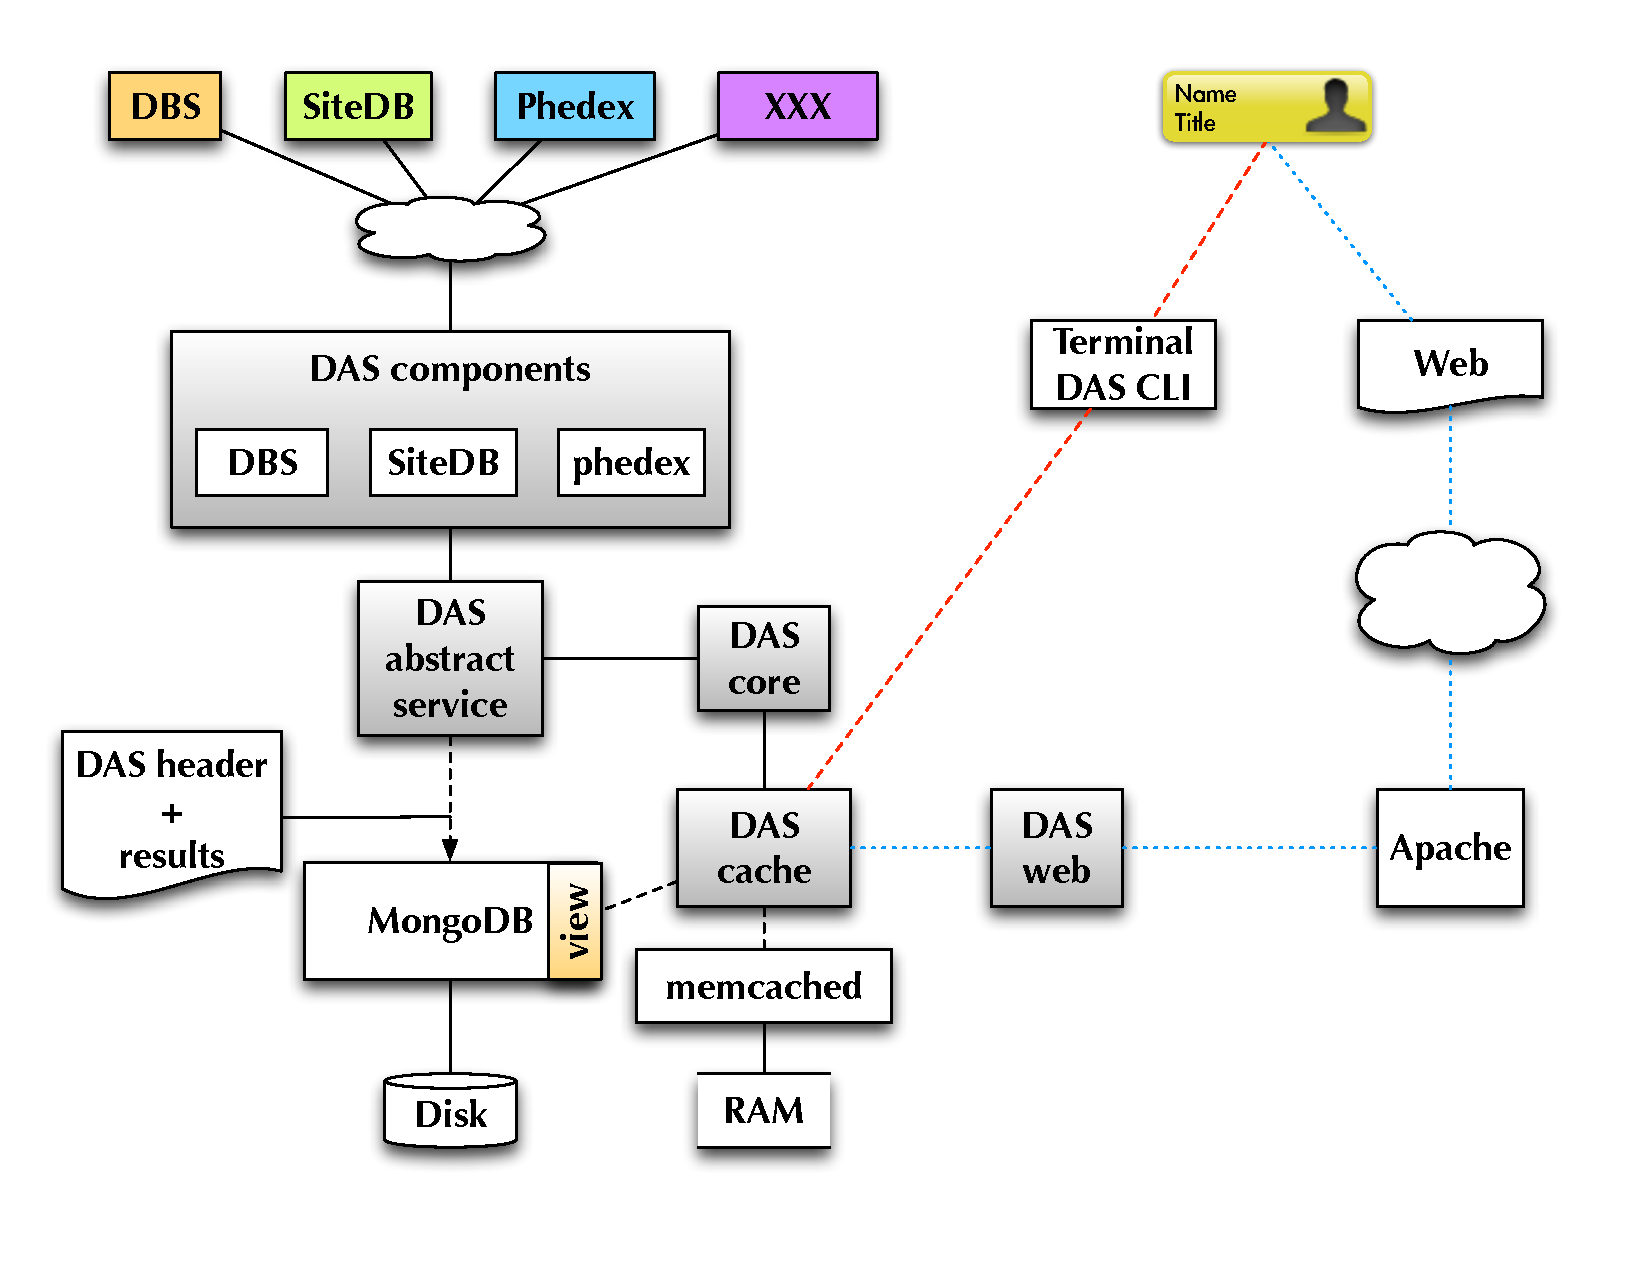
\includegraphics[width=150mm]{DAS_architecture.pdf}
%\caption{
%DAS architecture.
%}
%\label{DAS_arch}
%\end{figure}
\begin{figure}[htb]
\centering
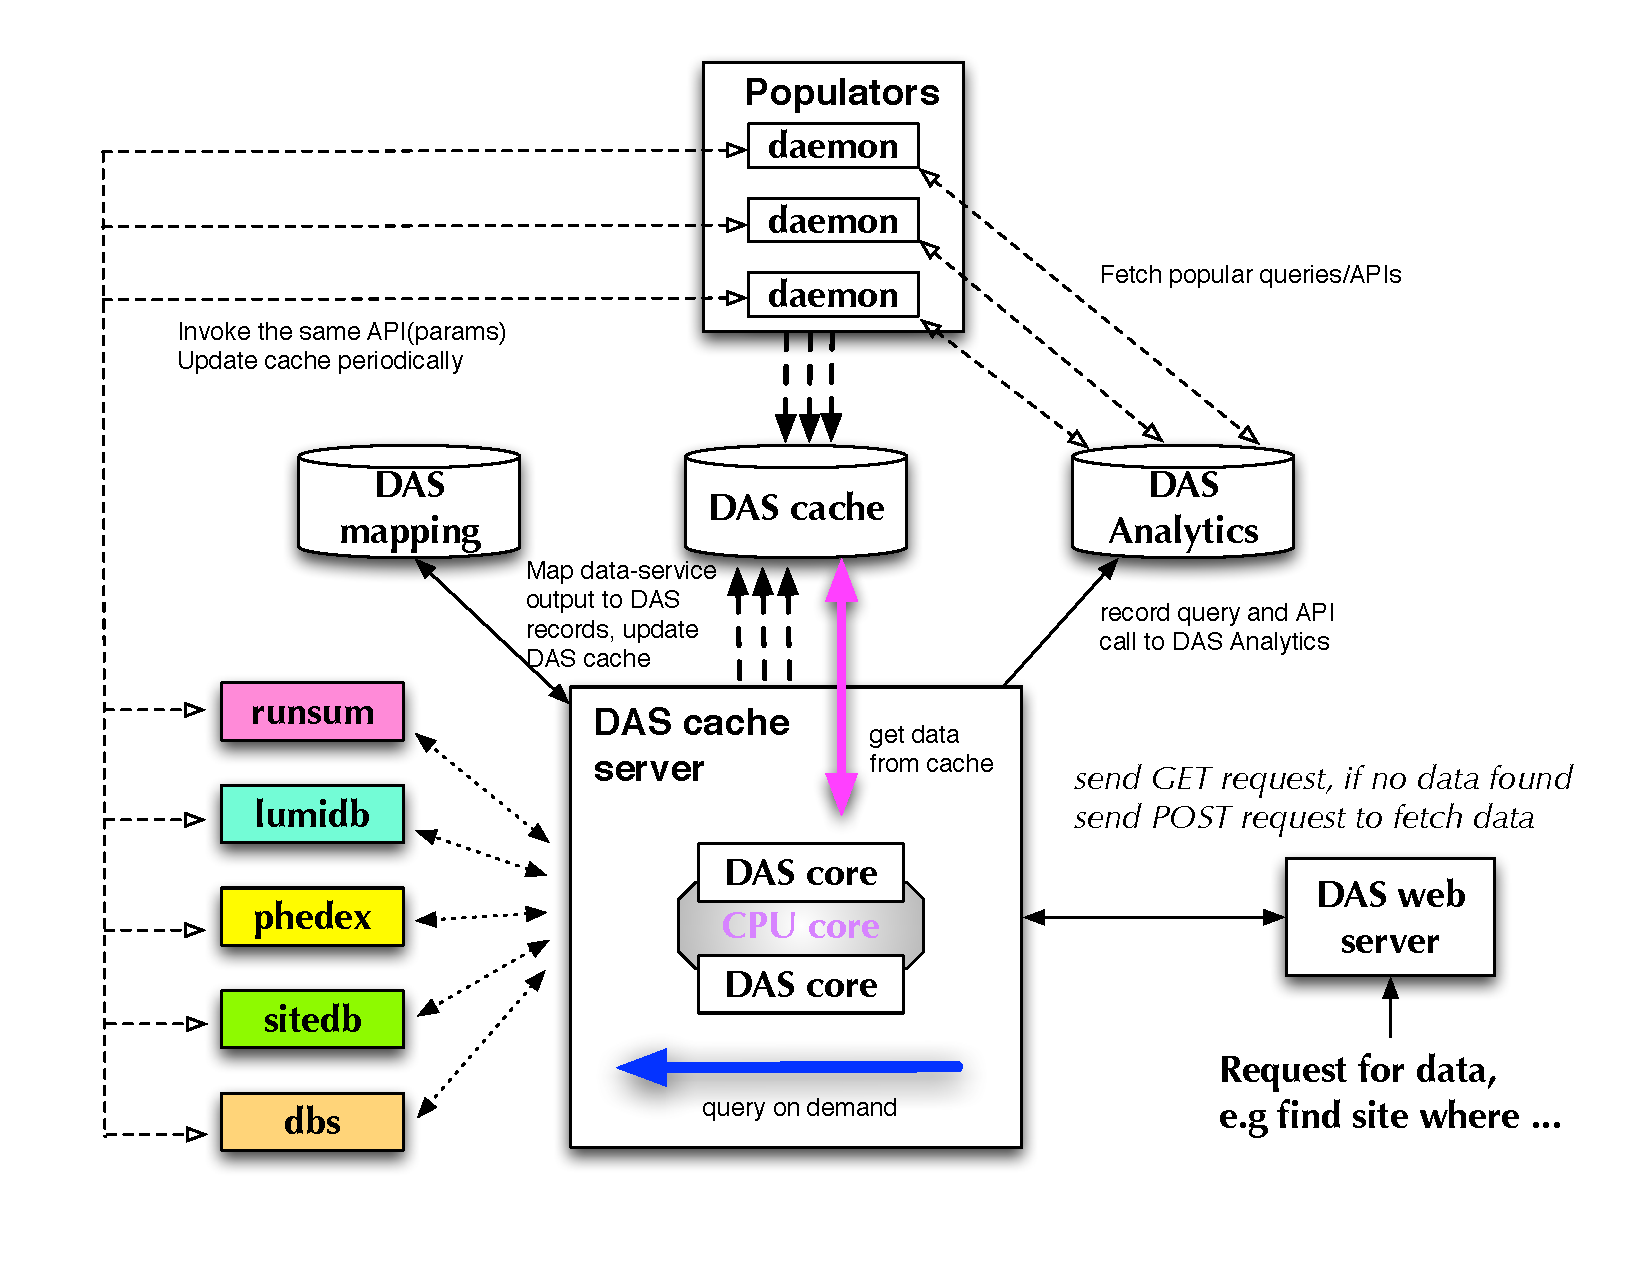
\includegraphics[width=150mm]{DAS_Cache_and_Analytics.pdf}
\caption{
DAS architecture diagram. It consists of DAS cache server, mapping and analytics DBs.
Once query was placed to DAS an associated
data-service API was invoked, triggering DAS cache population. Once data become
available in DAS cache user were able to see the results. This on demand
query retrieval system, where data were retrieved and store into cache from
back-end data service. We use DAS analytics DB to establish cache population
for most common queries by using DAS robots.
}
\label{DAS_cache}
\end{figure}

\noindent
Figure \ref{DAS_cache} summarize a overview of DAS architecture who consist of the
following components:
\begin{itemize}
\item DAS core library with support of pluggable modules for data retrieval;
\item DAS caching layer with long-term cache for aggregated results and short-term
cache for presentation layer;
\item DAS request service to handle user requests;
\item DAS mapping DB with DAS/data-services mapping, notations mapping and
mapping of DAS objects into data-presentation layer;
\item DAS analytics DB with query statistics to enable pre-fetching 
strategies.
\end{itemize}
Further we proceed with a discussion of individual DAS components.

\subsection{Dealing with data-services}
DAS provided pluggable system to add a new CMS data-service. To do that we
identify appropriate APIs, input and output parameters and keys, data-service
format and mapping between data-service, DAS and other sub-systems. 
This information were stored into DAS mapping DB. For instance,
the Data Bookkeeping System (DBS) and data location system (Phedex) both
provide information about CMS data files. In former case, DBS keeps information between
files and other physics  objects, such as run and luminosity, while Phedex provides 
information about file location, such as site and details about storage elements.
Upon user request to find information about a file, based on forementioned
information we were able to identify appropriate set of
data-service APIs, look-up data, re-format their output to DAS notations and
store results into DAS cache.\footnote{Even though we supported a data retrieval on demand
basis we also store user queries into DAS analytics DB to identify
a common patterns. Based on this information we organized a pre-fetching
strategies.}
Once data were retreived from data-services an additional step to aggregate
matched objects in DAS cache were applied. For instance in above examples
file information came from DBS and Phedex systems. 
Since both data-services output contained file name as a common
key, their output where merged and final result was stored into DAS cache.
This merged (aggregated) results represented a DAS data object. Each DAS data
object contains a standard DAS header, which identify look-up time,
request url, API, parameters and method as well as response version, expiration
time and checksum of the output. 

We designed DAS interface to be fully REST complaint \cite{REST}. It is not
only simplify development of DAS clients (CLI, web interface, robot, etc.)
but also consider DAS itself as own sub-component, i.e. place queries against
DAS content, rather then data-service one.

\subsection{Query Language\label{DAS-QL}}
Upon success of DBS-QL \cite{DBS-QL} we adopted its syntax to DAS with a few minor
changes. Here we briefly recall its syntax:
\begin{equation}
action\,\,\,
key_1,\, key_2,\, ...\,\,\, where\,\,\,
\langle key\rangle\, 
\langle op\rangle\, 
\langle value\rangle \,\,\, and|or ...
\label{QL_syntax}
\end{equation}
Each DAS QL expression starts with special keyword indicating an action such as 
$find,\, plot,\, summary$, followed by a set of selection keys. The action identify
the behavior of the query, find to look-up data, plot to plot found data, summary to
apply a summary view over provided selection keys. An optional conditions can be 
specified via $where$ keyword following by condition expression.
Each condition expression represented via $key\,\,\, operator\,\,\, value$ triplet, where
$key$ is DAS selection key, $operator$ is conditional operator, 
$=,\, >=,\, <,\, in,\, between$ and $value$ is a value applied to selection key.
We also support brackets as well as $and$ and $or$ logical operators.
The DAS selection and condition keys were identified based on analysis 
of terminology used by our users. For instance, $file$ was used to either
select file name or used in condition to identify file name provided by user.
Here is a simple example of DAS QL expression:
$$
find\,\,\, file,\, run\,\,\, where\,\,\, site=T1\_CH\_CERN
$$
which represents a natural language question: 
{\it find files and runs located at T1\_CH\_CERN site}.

\subsection{Mapping}
As been discussed above we used a DAS mapping DB to map data-service API into
DAS as well as map provide a relations between different data-services.
Upon identification of APIs which participate in DAS activity 
we store a mapping between data-service notations
into DAS mapping DB. This allows to map user input query parameters into
data-service API metrics as well as map back data-service output into DAS names.
For instance, the DBS system used $logical\_file\_name$ notation, while in Phedex
the same entity was named as $lfn$. Since both of them were referred to
logical file name, we map both notations into $file$ notation in DAS.\footnote{We
also deal with physical file names, but still used $file$ to refer to them in
DAS notation, since simple regular expressions were used to identify $file$
meaning from the provided value.}
For each service we provide a mapping from its own data-format (JSON, XML, etc.) into
common data-format used in DAS.\footnote{We used JSON as a DAS data format}
We also store a mapping between DAS keywords and data-service API names to
establish appropriate calls to data-service upon provided DAS query. For example,
when user specifies $file$ in their DAS query, we invoke DBS listFiles and Phedex
fileReplicas APIs. Since all mapping kept in RDMS we were able to abstract the 
DAS core library calls from hard coded data-service API calls and make it
transparent to any participating data-services. Here is a logic of DAS core
library:
\begin{itemize}
\item parse input DAS query
\item map provided selection and condition keys into data-service APIs and
input parameters
\item invoke data-service APIs
\item parse output results by mapping output notation into DAS keys
\item store and aggregate them into DAS raw-cache
\end{itemize} 


\subsection{Caching system and Analytics}
The DAS caching system was divided into two different caches: raw-cache and hot-cache.
The purpose of raw-cache was to store results coming from data services for
as long as specified in data-service response header. While the purpose of hot-cache
was to keep final DAS results corresponding to provided user query. We use a robot
services (jobs) to feed raw-cache with highly requested queries. Here we will only
discuss the raw-cache organization. 
%\begin{figure}[htb]
%\centering
%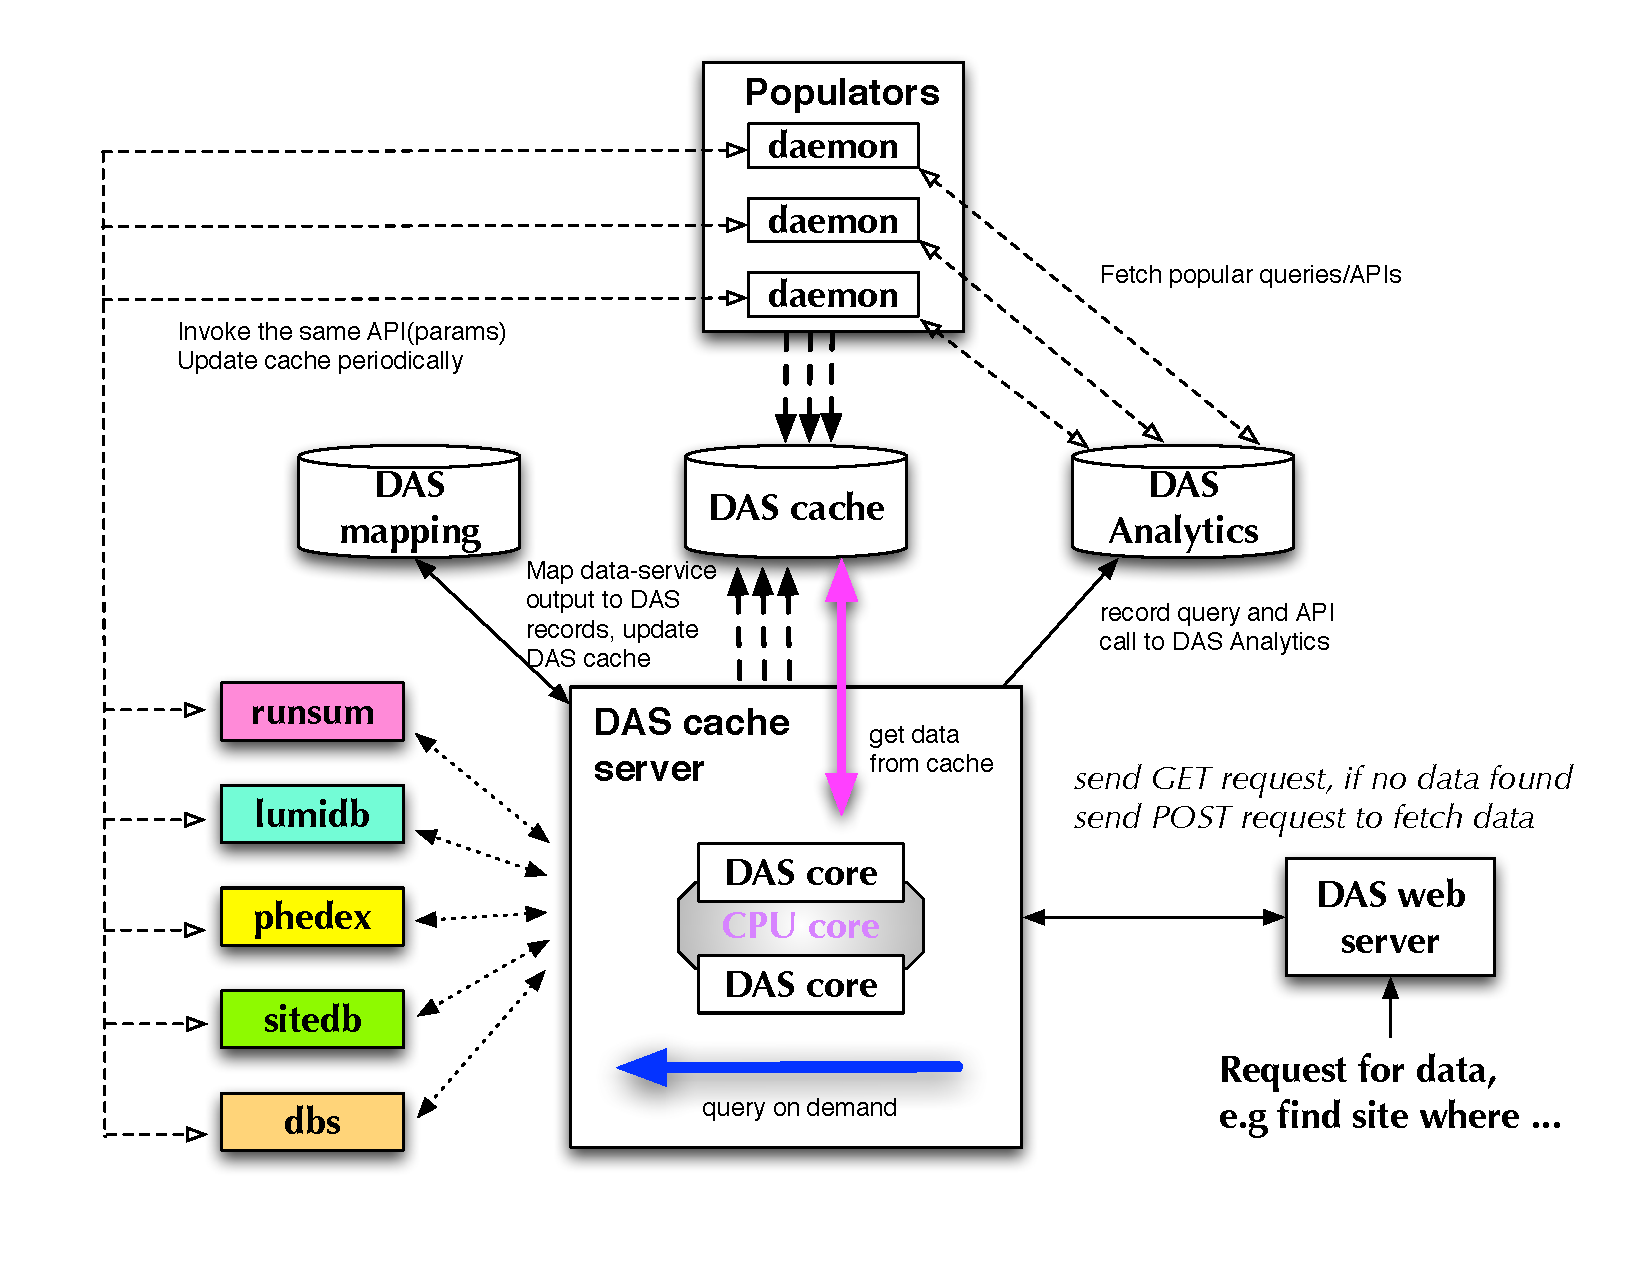
\includegraphics[width=150mm]{DAS_Cache_and_Analytics.pdf}
%\caption{
%DAS cache system.
%}
%\label{DAS_cache}
%\end{figure}
As it shown in figure \ref{DAS_cache} the DAS cache server has dual purpose.
On one side it talks to DAS Analytics DB to trigger jobs for worker robot
who update cache with most popular queries, on another it talks to DAS
raw-cache back-end to either stored mapped results or merge them with 
existing DAS objects in a cache. We should note that we use on-demand
approach to answer user queries, but at the same time with a help of
DAS Analytics DB we force worker robots (robots) to pre-fetch
the most popular queries up-front.

We evaluated several technologies
as a choice for DAS cache back-end, including relational MySQL DB \cite{MySQL} 
and object oriented CouchDB \cite{CouchDB} and MongoDB \cite{MongoDB}.
Each of them had its own pros and cons. For instance usage
of MySQL provided a SQL queries (as in federated DBs, see \cite{FedDB}), but
required auto-schema generation on a fly.\footnote{We did not apply any
restriction to DAS QL and did not know in advance what our users will be
querying.} While, using CouchDB and MongoDB, we were able to store
data-service output naturally as documents objects into DB. Finally we decided
to use MongoDB due to its flexible and
powerful querying syntax, which were easy to map into DAS QL expressions. 

\section{Results\label{Results}}
DAS was deployed with the following CMS data-services:
\begin{itemize}
\item DBS \cite{DBS}, Data Bookkeeping System which collect information
about CMS meta-data;
\item PhEDEx \cite{Phedex}, Physics Experiment Data Export project which
provides the data placement and the file transfer system for the CMS experiment;
\item RunSummary DB \cite{RunSummary} collects information about run and triggers
conditions during data-taking;
\item LumiDB \cite{LumiDB} collects information about Luminosity conditions;
\item DQ \cite{DQ}, Data Quality data-service which collects information
about detector conditions during data taking;
\item Overview \cite{Overview}, collects information about CMS
transfer rate, etc.;
\item Dashboard \cite{Dashboard} project for LHC experiments aims to 
provide a single entry point to the monitoring data collected from the 
distributed computing systems of the LHC virtual organization.
\end{itemize}
Each data-service has its own scope, size and lifetime. For instance the data
in Phedex are transient due to constant migration of CMS data. The DBS system
were divided into dozen of individual DBs, whose size varied at the level of
few tens of GBs.

\section{Summary}

\section{Acknowledgments}

This work was supported by the National Science Foundation and Department of Energy of the United States of America. Fermilab is operated by Fermi Research Alliance, LLC under Contract
No. DE-AC02-07CH11359 with the United States Department of Energy.

\section*{References}
\begin{thebibliography}{9}
\bibitem{Arms}
C. R. Arms, W. Y. Arms, ``Mixed Content and Mixed Metadata 
Information Discovery in a Messy World'',
chapter from ``Metadata in Practice'', ALA Editions, 2004

\bibitem{FedDB}
L. Haas, E. Lin,
``IBM Federated Database Technology'', \\
http://www.ibm.com/developerworks/data/library/techarticle/0203haas/0203haas.html

\bibitem{DBXplorer}
Sanjay Agrawal, Surajit Chaudhuri, Gautam Das: DBXplorer: A System for
Keyword-Based Search over Relational Databases. ICDE 2002: 5-16

\bibitem{QueryAnswer}
Georgia Koutrika, Alkis Simitsis, Yannis E. Ioannidis: Pr\'{e}cis: The Essence of
a Query Answer. ICDE 2006: 69-78

\bibitem{DBS-QL} V. Kuznetsov, D. Riley, A. Afaq, V. Sekhri, Y. Guo, L. Lueking,
``The CMS DBS Query Language'', CHEP 2009

\bibitem{CMSDataModel} A. Fanfani et. al.,
``Distributed Analysis in CMS'', to be published in Journal of Grid Computing.

\bibitem{DBS} A. Afaq, et. al. ``The CMS Dataset Bookkeeping Service'', CHEP 2007 

\bibitem{DBS07} A. Dolgert, V. Kuznetsov, C. Jones, D. Riley, 
``A multi-dimensional view on information retrieval of CMS data'', CHEP 2007

\bibitem{DD} https://cmsweb.cern.ch/dbs\_discovery

\bibitem{MySQL}
http://www.mysql.com/

\bibitem{CouchDB}
http://couchdb.apache.org/

\bibitem{MongoDB}
http://www.mongodb.org/

\bibitem{REST}
Fielding, Roy Thomas ``Architectural Styles and the Design of 
Network-based Software Architectures'', Doctoral dissertation, 2000,
University of California, Irvine

\bibitem{Phedex}
Rehn et. al.,
``PhEDEx high-throughput data transfer management system'', CHEP06, Mumbai, India.

\bibitem{RunSummary}

\bibitem{SiteDB}

\bibitem{LumiDB}
https://twiki.cern.ch/twiki/bin/view/CMS/CMS-DMWM-DBS-Luminosity

\bibitem{DQ}

\bibitem{Overview}
https://cmsweb.cern.ch/overview/

\bibitem{Dashboard}
J. Andreeva, et. al,
``Experiment Dashboard – The Monitoring System for the LHC Experiments'',
GMW’07, June 25, 2007, Monterey, California, USA.

\bibitem{DBSearch}
D. Konopnicki, O. Shmueli,
``Database-Inspired Search'', 
Proc. of the 31st VLDB Conference, 2005.
\end{thebibliography}

\end{document}


